\section{Die EV3-Steuereinheit}
	\begin{figure}[h]
		\begin{floatrow}
			\ffigbox{%
				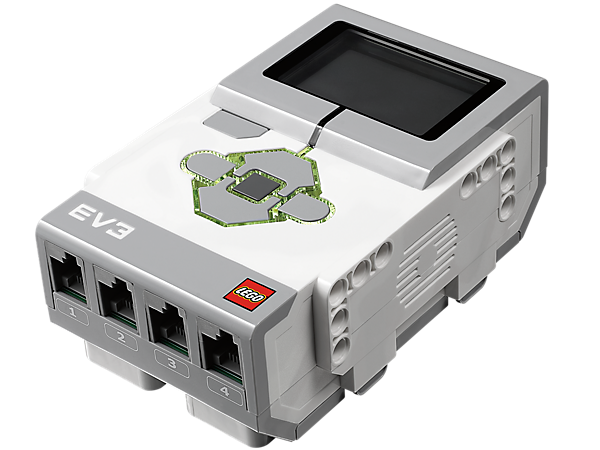
\includegraphics[width=9cm]{images/brick.png}%\rule{3cm}{3cm}%
			}{%
				\caption{EV3-Brick}%
			}
			\capbtabbox{%
				\footnotesize
				\begin{tabular}{|c|c|} \hline
					Motorausg"ange & MotorPort.A \\
					&MotorPort.B\\
					&MotorPort.C\\
					&MotorPort.D\\ \hline
					Links & LEFT \\ \hline
					Rechts & RIGHT \\ \hline
					Oben & UP \\ \hline
					Unten & DOWN \\ \hline
					Mitte & ENTER \\ \hline
					Oben-Links & ESCAPE \\ \hline
					Sensoreing"ange & SensorPort.S1 \\
					&SensorPort.S2\\
					&SensorPort.S3\\
					&SensorPort.S4\\ \hline
				\end{tabular}
			}{%
				\caption{Tastenbenennung}%
			}
		\end{floatrow}
	\end{figure}
	
	Durch Dr"ucken der mittleren und unteren Taste wird das laufende Programm beendet.
	

